\chapter{Methodik}

\section{Vorgehensmodell}

\subsection{\ac{GQM}}

Befragung Team blabla

\subsubsection{Vorauswahl}

Um eine Vorauswahl an Metriken treffen zu können, wurden alle bisherigen Retrospektiven (es waren genau 15) analysiert und eine Topliste von Schlagwörtern der folgenden Fragestellungen aus den Retrospektiven erstellt:
\begin{enumerate}
    \item Welche guten Entscheidungen haben wir getroffen?
    \item Was haben wir gelernt?
    \item Was können wir besser machen?
    \item Was nervt uns noch immer?
\end{enumerate}

Dazu wurden die Ergebnisse in eine ElasticSearch Datenbank gespeichert und über eine sogenannte Terms Aggregation die wichtigsten Schlagwörter analysiert.
Bei der Indizierung werden die Wörter normalisiert, deshalb die teilweise andere Schreibweise (zum Beispiel wird aus Issue der Term issu).
\newline
Aus den Ergebnissen in Anhang~\ref{appendix:retros} ist ersichtlich, dass

\section{Software}

Technologien, Plattform, etc.

\subsection{Architektur}

Abbildung~\ref{fig:position_architecture} zeigt die Position und Abbildung~\ref{fig:overview_architecture} die grobe Architektur der Software (Agile Metrics).
Die Software bildet eine Schnittstelle zwischen den einzelnen Systemen des Entwicklungsprozesses und dem System zur Darstellung der Metriken (in diesem Fall ElasticSearch und Kibana).

\begin{savenotes}
    \begin{figure}[H] 
        \centering
            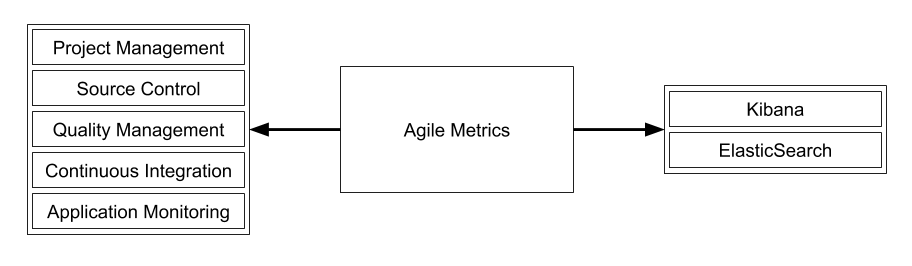
\includegraphics[width=0.8\textwidth]{img/position-overview.png}
        \caption{Position der Software}\label{fig:position_architecture}
    \end{figure}
\end{savenotes}

\begin{savenotes}
    \begin{figure}[H] 
        \centering
            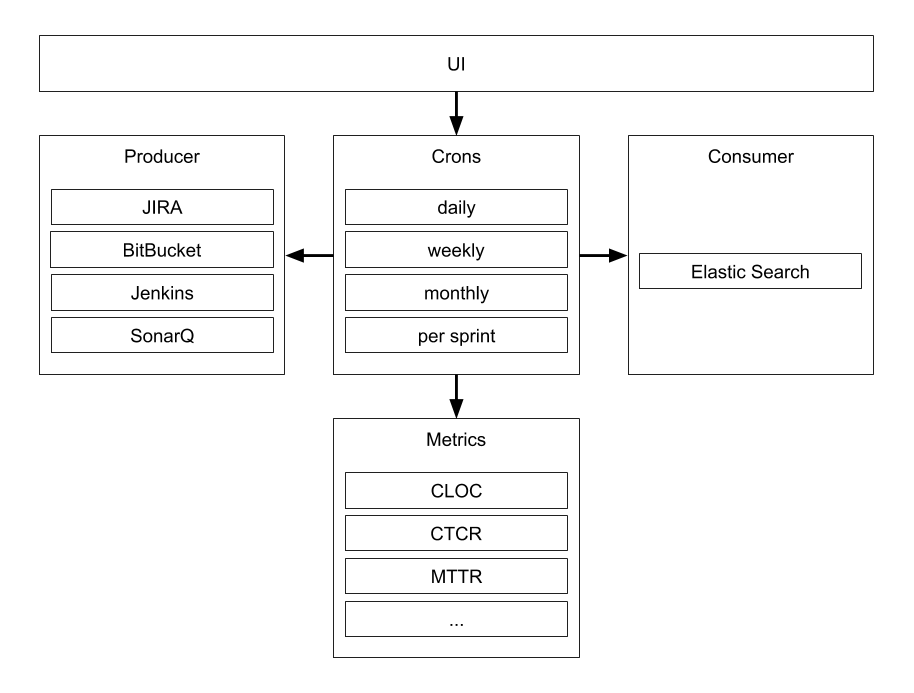
\includegraphics[width=0.8\textwidth]{img/architecture-overview.png}
        \caption{Übersicht der Software-Architektur}\label{fig:overview_architecture}
    \end{figure}
\end{savenotes}

\begin{description}
    \item[UI] \hfill \\ Bietet eine grafische Benutzeroberfläche zur Konfiguration.
    \item[Producer] \hfill \\ Sind Schnittstellen zu allen Systemen, die Messdaten erzeugen.
    \item[Crons] \hfill \\ Zeitsteuerung der Messdaten-Abfrage (z.B. täglich oder pro Sprint).
    \item[Metrics] \hfill \\ Hier können aus Messdaten direkt Metriken erstellt werden.
    \item[Consumer] \hfill \\ Sind Schnittstellen zu allen Systemen, die Messdaten und Metriken konsumieren.
\end{description}
